\documentclass[xcolor=pdftex,dvipsnames,table]{beamer}
\usetheme{Darmstadt}
\usepackage{etex}
\providecommand\thispdfpagelabel[1]{}
\usepackage[latin1]{inputenc}
\usepackage{amsmath}
\usepackage{amssymb}
\usepackage{amsthm}
\usepackage{listings}
\usepackage{graphics}
\usepackage{framed}
\usepackage{etex}
\usepackage[all]{xy}
\usepackage{xspace,listings,ulem,tikz}
\usepackage[outline]{contour}
\contourlength{1.2pt}
\usepackage[square,sort,comma,numbers]{natbib}
\setbeamertemplate{footline}[frame number]
\tikzset{
    onslide/.code args={<#1>#2}{% http://tex.stackexchange.com/a/6155/16595
        \only<#1>{\pgfkeysalso{#2}}
    },
    hideshow/.style args={<#1><#2>#3}{%
        onslide=<#1>{move to},
        onslide=<#2>{#3}
    }
}
\lstset{
         basicstyle=\footnotesize\ttfamily, % Standardschrift
         %numbers=left,               % Ort der Zeilennummern
         numberstyle=\tiny,          % Stil der Zeilennummern
         %stepnumber=2,               % Abstand zwischen den Zeilennummern
         numbersep=5pt,              % Abstand der Nummern zum Text
         tabsize=2,                  % Groesse von Tabs
         extendedchars=true,         %
         breaklines=true,            % Zeilen werden Umgebrochen
         keywordstyle=\color{red},
    		frame=b,         
 %        keywordstyle=[1]\textbf,    % Stil der Keywords
 %        keywordstyle=[2]\textbf,    %
 %        keywordstyle=[3]\textbf,    %
 %        keywordstyle=[4]\textbf,   \sqrt{\sqrt{}} %
         %stringstyle=\color{white}\ttfamily, % Farbe der String
         showspaces=false,           % Leerzeichen anzeigen ?
         showtabs=false,             % Tabs anzeigen ?
         xleftmargin=3pt,
         framexleftmargin=3pt,
         framexrightmargin=1pt,
         framexbottommargin=3pt,
         language=C++,
         %backgroundcolor=\color{lightgray},
         showstringspaces=false      % Leerzeichen in Strings anzeigen ?        
 }

 \usetikzlibrary{arrows}
 \usepackage{caption}
\DeclareCaptionFont{white}{\color{white}}
\DeclareCaptionFormat{listing}{\colorbox[cmyk]{0.43, 0.35, 0.35,0.01}{\parbox{\textwidth}{\hspace{15pt}#1#2#3}}}
\captionsetup[lstlisting]{format=listing,labelfont=white,textfont=white, singlelinecheck=false, margin=0pt, font={bf,footnotesize}}
\beamertemplatenavigationsymbolsempty
\newcommand{\N}{\ensuremath{\mathbb{N}}} 
\newcommand{\R}{\ensuremath{\mathbb{R}}} 
\newcommand{\RR}{\ensuremath{\mathbb{R}}} 
\newcommand{\C}{\ensuremath{\mathbb{C}}} 
\newcommand{\Q}{\ensuremath{\mathbb{Q}}} 
\newcommand{\Z}{\ensuremath{\mathbb{Z}}} 
\newcommand{\D}{\ensuremath{\mathbb{D}}}
\newcommand{\lb}{\mathrm{lb}}
\newcommand{\dy}{\mathrm{dy}}
\newcommand{\cc}{\texttt{C++}\xspace}
\newcommand{\bin}{\mathrm{bin}}
\newcommand{\irram}{\texttt{iRRAM}\xspace}
\newcommand{\code}[1]{\texttt{#1}}
\newcommand{\sharpp}{\ensuremath{\#\mathcal P}\xspace}
\newcommand{\sharppu}{\ensuremath{\#{\mathcal P}_1}\xspace}
\newcommand{\fp}{\ensuremath{\mathcal{FP}}\xspace}
  \newcommand{\baana}{\code{BA\_ANA}\xspace}
  \newcommand{\anarect}{\code{ANA\_RECT}\xspace}
  \newcommand{\powerseries}{\code{POWERSERIES}\xspace}
  \newcommand{\poly}{\code{POLY}\xspace}
  \newcommand{\func}{\code{FUNC}\xspace}
  \newcommand{\real}{\code{REAL}\xspace}
  \newcommand{\complex}{\code{COMPLEX}\xspace}
  \newcommand{\temp}{\textcolor{red}}
  \newcommand{\seq}{\mathbf}
\newcommand{\fpu}{\ensuremath{\mathcal{FP}_1}\xspace}
\DeclareMathOperator{\dom}{\mathrm{dom}}
\newtheorem{conjecture}{Conjecture} 
\newtheorem{representation1}{Representation 1} 
\newtheorem{representation1b}{Representation 1'} 
\newtheorem{representation2}{Representation 2} 
\title[Analytic Continuation in iRRAM]{Analytic Continuation in \irram}
\author[A. Kawamura, F. Steinberg, H. Thies]{
		Akitoshi Kawamura, Florian Steinberg, Holger Thies 
}
\institute[Theorietag]{
  69. Workshop \"{u}ber Algorithmen und Komplexit\"{a}t, Technische Universit\"{a}t Ilmenau
}
\begin{document}
\setbeamercolor{note}{fg=black,bg=lightgray} 
\date{May 28, 2015}
\frame{
\titlepage
}
\frame[<+->]{
\frametitle{Table of Contents}
\tableofcontents
}
\section{Background}
\begin{frame}
	\frametitle{Algorithm Engineering}
	\centering
	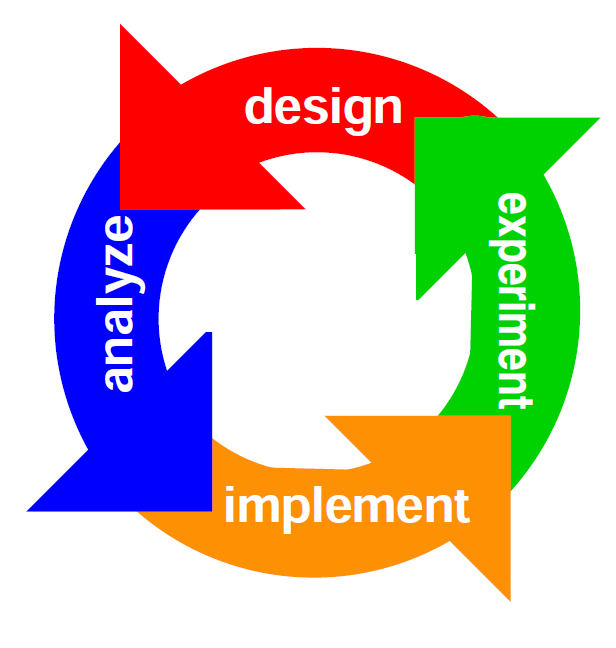
\includegraphics[width=0.7\textwidth]{approach.png}
\end{frame}
\begin{frame}[<+->]
\frametitle{iRRAM}
\begin{itemize}[<+->]
\item iRRAM is a C++ framework for exact real computations
\item Ordinary C++ is extended by datatype REAL for computing with real numbers
\item Usual arithmetic operations are implemented for REAL
\item Other functions like abs, power, root, modulo, exp, log, sin, cos are also available
\end{itemize}
\end{frame}
\begin{frame}
  \frametitle{\irram: Real Number Representation}
  \centering
    \begin{tikzpicture}[remember picture, overlay]
     \node[font=\huge] at (0,0) {$x \in [\textcolor{green}{d}-\textcolor{red}{e},\textcolor{green}{d}+\textcolor{red}{e}]$};
     \draw<2-> [->, line width=3pt,color=green] (-1,0.4) -- (-1,2);
     \node<2->[color=green,font=\large] at (-1,2.2) {Multiple precision floating point number};
     \draw<3-> [->, line width=3pt,color=red] (2.4,-0.4) -- (2.4,-2);
     \node<3->[color=red,font=\large] at (2.4,-2.2) {$e = z \cdot 2^p$ (p,z \code{long})};
    \end{tikzpicture}
\end{frame}

\begin{frame}[<+->][fragile]
\frametitle{Example: \irram}
\begin{example}
\begin{lstlisting}
REAL series(int n){
  return power(REAL(2), -n);
}
REAL xinv_approx(long p, REAL& x){
  int N=-2*p+3;
  REAL ans = 0.0;
  for(int i=0; i<=N; i++)
    ans += series(i)*power(x,i);
  return ans;
}
REAL xinv(REAL& x) { return limit(xinv_approx, x);}
\end{lstlisting}
\end{example}
\end{frame}


\subsection{Analytic Functions}
\begin{frame}
\frametitle{Analytic Functions and Computational Complexity}
\begin{fact}
For general polynomial time computable functions, many important operators have been shown to be computationally hard.\\
For example
\begin{itemize}[<+->]
\item Polynomial time computable functions may have noncomputable derivatives. (Ko 1983)
\item Parametric maximization is NP-hard. (Ko/Friedman (1982))
\item Integration is \#P-hard. (Friedman (1984))
\end{itemize}
\end{fact}
\pause
We want to find a subset of polynomial time computable functions on which we can perform those operations in polynomial time.
\end{frame}
\begin{frame}
\frametitle{Analytic Function}
An analytic function is a function locally given by a complex power series.\\
\begin{definition}[Analytic Function]
% \begin{columns}
% \begin{column}{0.4\linewidth}
$f : D \to \C $, $D \subseteq \C$ is analytic if for any $x_0 \in D$ the Taylor-series
$$ T(x) := \sum^\infty_{n=0} a_n(x-x_0)^n$$
converges to $f(x)$ for $x$ in a neighborhood of $x_0$.  
% \end{column}
% \begin{column}{0.4\linewidth}
% 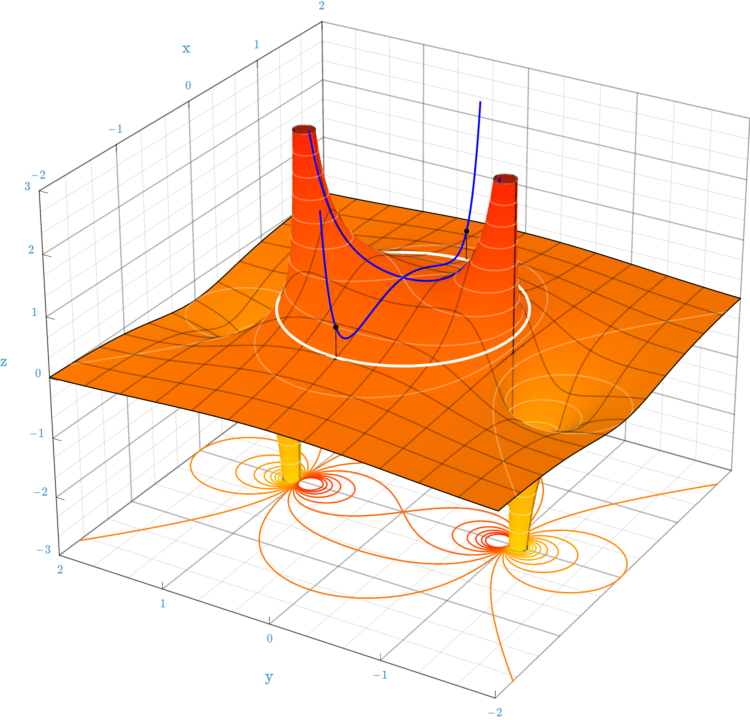
\includegraphics[width=4.5cm]{TaylorComplexConv}
% \end{column}
% \end{columns}
\end{definition}
\end{frame}
\begin{frame}
\frametitle{Some non-uniform results}

$$a_m =\frac{f^{(m)}(x_0)}{m!} 
, \,\, f(x) = \sum_{m=0}^\infty a_m(x-x_0)^k \,\ \text{ for } x \in B(x_0,R)
$$
\vfill
\begin{theorem}[Pour-El, Richards, Ko, Friedman, M\"uller (1987/1989)]
$f$ is (polytime) computable iff $(a_m)_{m \in \N}$ is.
\end{theorem}
 \onslide<2->{
From that polynomial time computability of the derivative and the anti-derivative of a function follows immediately.
}
\end{frame}
\begin{frame}
\frametitle{Some non-uniform results}
$$a_m =\frac{f^{(m)}(0)}{m!} 
, \,\, f(x) = \sum_{m=0}^\infty a_mx^k \,\ \text{ for } x \in B(0,R)
$$
\vfill
\begin{theorem}[M\"uller (1995)]
\begin{itemize}
\item The operator $f \to (a_m)_{m \in \N}$ is not computable.
\item The evaluation operator $((a_m)_{m \in \N},x) \to f(x) $ is not computable.
\end{itemize}
\end{theorem}
\pause
However, if we supply some additional (discrete) information those operators become computable.
\end{frame}


\subsection{Representing power series}
\begin{frame}
\frametitle{A practical representation for power series}
\begin{lemma}
Let $f : \C \to \C$ be analytic on the closed unit disc and $(a_m)_{m\in\N}$ its Taylor series around $0$.\\
Then $R>1$ \pause and we can find two positive integers $k$ and $A$ with 
\begin{itemize}
\item $r := \sqrt[k]{2}$ is strictly smaller than the radius of convergence $R$.
\item $|a_m|r^m \leq A$ for all $m \in \N$.
\end{itemize}
\end{lemma}
\pause
With $k$ and $A$ we can estimate 
$$ \left | \sum_{n \geq N} a_m z^n \right | \leq A\frac{(|z|/r)^N}{1-|z|/r} $$\pause
Consider triples $\big((a_m)_{n \in \N}, k, A\big)$ as representation for functions analytic on the unit disc.
\end{frame}
%\begin{frame}
%\frametitle{Finding $k$ and $A$}
%\begin{itemize}
%\item Choose $k$ appropriately and let $r := \sqrt{k}{2}$
%\item $f_{|z|=r}$ is a continuous function on a compact domain, thus is bounded by some number $A$
%\item By Cauchy Differentiation formula $$|a_n| \leq |\frac{1}{2\pi i}\int_{z=|r|} \frac{f(z)}{|z|^{n+1}} d \lambda| \leq \frac{A}{r^n}$$
%\end{itemize}
%\end{frame}
\begin{frame}[<+->]
\frametitle{Analytic Functions and Computational Complexity}
\begin{theorem}[Kawamura, R\"osnick, M\"uller, Ziegler (2013)]
  The following operators are computable in time polynomial in $k+log(A)+n$, where $2^{-n}$ is the output precision.
\begin{enumerate}
\item evaluation
\item addition and multiplication
\item differentiation and anti-differentiation
\item parametric maximization
\end{enumerate}
\end{theorem}
\end{frame}
\begin{frame}
\frametitle{\small Analytic functions on $[-1,1]$ (Kawamura, R\"osnick, M\"uller, Ziegler (2013))}
We want to consider complex functions analytic on $[-1,1]$.\\ 
\begin{minipage}{0.45\textwidth}
\begin{center}
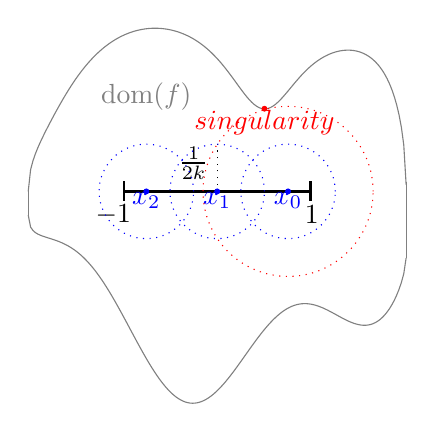
\begin{tikzpicture}[scale=0.6]
%    \draw<3> (-1,1) rectangle (5,-1);
    \node<1->  at (-0.2,-0.5) {$-1$};
    \node<1->  at (4.0,-0.5) {$1$};
    \draw<1-> [thick,|-|] (0,0) -- (4,0);
    \node<2>  at (1.5,.6) {$\frac 1{2k}$};
    \draw<2>  [dotted] (2.0,0) -- (2.0,1);
%    \node<3>  at (-.7,-.25) {$\frac 1l$};
%    \draw<3>  [dotted] (-1,0) -- (0,0);
%    \node<3>  at (2.2,.5) {$\frac 1l$};
%    \draw<3>  [dotted] (2,1) -- (2,0);
%    \node<3>  at (-.5,0.6) {$\overline R_l$};
    \draw<1-> [domain = 0:8,color=gray] plot[samples=160] (\x-2, {sqrt(16-(\x-4)^2)*(1-1/(\x^2+1) + sin(\x) + (\x/7)^5-\x/6 +1.5- 1/((\x-5)^2+1))/2});
    \draw<1-> [domain = 0:8,color=gray] plot[samples=160] (\x-2, {1/(\x^2+1)/2 + sin(80*\x) + (\x/7)^5-\x/6 -1-sqrt(16-(\x-4)^2)/2});
    \draw<1-> [color=gray] (-2,0) -- (-2,-.5);
    \draw<1-> [color=gray] (6,.19) -- (6,-1.42);
    \node<1-> [color=gray] at (.5,2) {$\dom(f)$};
    \draw<2> [fill=blue,radius =.05,color=blue] (3.5,0) circle;
    \node<2> [color=blue] at (3.5,-.2) {$x_0$};
    \draw<2> [fill=blue,radius =.05,color=blue] (2.0,0) circle;
    \node<2> [color=blue] at (2.0,-.2) {$x_1$};
    \draw<2> [radius = 1,color=blue, dotted] (2.0,0) circle; 
    \draw<2> [fill=blue,radius =.05,color=blue] (0.5,0) circle;
    \node<2> [color=blue] at (0.5,-.2) {$x_2$}; 
    \draw<2> [radius = 1,color=blue, dotted] (0.5,0) circle;
    \draw<2> [radius = 1,color=blue, dotted] (3.5,0) circle;
    \draw<2> [radius = 1.8, color = red, dotted] (3.5,0) circle; 
    \draw<1-> [fill=red,radius = .05,color = red] (3,1.75) circle;
    \node<1-> [color=red] at (3,1.45) {$singularity$};
    %\draw<3> [radius = 1, color = green, dotted] (2.5,0) circle;
    %\draw<3> [fill=green, radius = .05, color = green] (2.5,0) circle;
    %\node<3> [color=green] at (2.5,-.2) {$x_1$};
\end{tikzpicture}
\end{center}
\end{minipage}
\hfill
\begin{minipage}{0.45\textwidth}
\onslide<2->{
\begin{representation1}
  A finite number of taylor series together with parameters $A$ and $k$ that hold for each series, such that they cover the domain. 
 \end{representation1}
}
% \onslide<3->{
%\begin{representation2}
%A tuple $\big(f|_{[-1,1]}, B, l\big)$, $f \in C^\omega(\overline R_l)$ and $|f|_{\overline R_l}| \leq B$ where $\overline R_l := [-1-\frac1l,1+\frac1l]x[-\frac1l, \frac1l]$  
%\end{representation2}
%}
\end{minipage}
\end{frame}
%\begin{frame}
%\begin{minipage}{0.45\textwidth}
%\begin{representation1}
%A tuple $(M, (x_m), (a_{m,j}), A,k)$ $1 \leq m \leq M$, $j \in \N$ s.t. % with $1 \leq m \leq M$, $j \in \N$ so that
%%\item $a_{m,j}$ describes a Taylor series for $f$ around $x_m$ 
%$[-1,1] \subseteq \bigcup [x_m-\frac{1}{4k}, x_m+\frac{1}{4k}]$ \\
%and $|a_{m,j}| \leq A \cdot k^j$
% \end{representation1}
% \end{minipage}
% \hfill
% \begin{minipage}{0.45\textwidth}
%\begin{representation2}
%A tuple $\big(f|_{[-1,1]}, B, l\big)$, $f \in C^\omega(\overline R_l)$ and $|f|_{\overline R_l}| \leq B$ where $\overline R_l := [-1-\frac1l,1+\frac1l]x[-\frac1l, \frac1l]$  
%\end{representation2}
%\end{minipage}
%\begin{theorem}[Kawamura, R\"osnick, M\"uller, Ziegler (2013)]
%\begin{itemize}[<+->]
%\item Given $(M, (x_m), (a_{m,j}), A,k)$ we can evaluate $f(x)$ in time polynomial in $n+k+\lb(A)$
%\item From $(f,B,l)$ we can compute $(f^{(j)}(x_0))_{j \in \N}$ in time polynomial in $n+\lb(l)+\lb(B)$ 
%%and for all $x \in [-1,1]$ $|f^{(j)}(x)| \leq B\cdot l^j \cdot j!$
%\end{itemize}
%\end{theorem}
%\pause
%This means we can convert between those two representations in (parametrized) polynomial time.
%\end{frame} 

%\begin{frame}[<+->]
%\frametitle{Computing Taylor series}
%\begin{itemize}
%\item To convert between those representations we have to compute the Taylor coefficients from a given function
%\item Described in detail in (M\"uller87)
%\item Want to approximate the coefficient $a_m$ with max. error $2^{-n}$
%\item Approximate $f$ by Lagrangian interpolating polynomial $P_m(x) := \sum_{i=0}^{2m} f(x_i) \cdot L_{m,i}(x)$ with $L_{m,i}(x) = \prod_{j \neq i} \frac{x-x_j}{x_i-x_j} $ and $x_i = (i-m)\cdot h$
%\item Differentiate this polynomial $P^{(m)}(0) = \sum_{i=0}^{2m} f(z_i)\cdot L_{m,i}^{(m)}(0)$
%\item $\frac{1}{m!}P^{(m)}(0) = \sum_{i=0}^{2m} f(x_i)\frac{h^{-m}\cdot l_{m,i}}{i!(2m-i)!}$ with integers $l_{m,i}$
%\item An error bound for this approximation can be computed
%\end{itemize}
%\end{frame}


\begin{frame}
\frametitle{Evaluation}
\begin{minipage}{0.45\textwidth}

\begin{representation1}
  A finite number of taylor series together with parameters $A$ and $k$ that hold for each series covering the domain.
 \end{representation1}


\begin{representation2}
  A \textbf{single} taylor series together with parameters $A$ and $k$ that are valid for the the taylor series around any point of the domain.
\end{representation2}
\end{minipage}
\hfill
\begin{minipage}{0.45\textwidth}
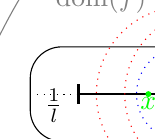
\begin{tikzpicture}[scale=0.6]
    \path [use as bounding box,red] (-30pt,-10pt) rectangle (30pt,40pt);
    \draw[rounded corners=4mm] (-1,1) rectangle (5,-1);
    %\draw (2,0) ellipse (3cm and 1cm);
    \draw [thick,|-|] (0,0) -- (4,0);
    \node at (-.5,-.25) {$\frac 1l$};
    \draw [dotted] (-1,0) -- (0,0);
    \node at (2.2,.5) {$\frac 1l$};
    \draw [dotted] (2,1) -- (2,0);
    \draw [domain = 0:8,color=gray] plot[samples=160] (\x-2, {sqrt(16-(\x-4)^2)*(1-1/(\x^2+1) + sin(\x) + (\x/7)^5-\x/6 +1.5- 1/((\x-5)^2+1))/2});
    \draw [domain = 0:8,color=gray] plot[samples=160] (\x-2, {1/(\x^2+1)/2 + sin(80*\x) + (\x/7)^5-\x/6 -1-sqrt(16-(\x-4)^2)/2});
    \draw [color=gray] (-2,0) -- (-2,-.5);
    \draw [color=gray] (6,.19) -- (6,-1.42);
    \node [color=gray] at (.5,2) {$\dom(f)$};
    \draw<1-3> [fill=blue,radius =.05,color=blue] (3.5,0) circle;
    \node<1-3> [color=blue] at (3.5,-.2) {$x_0$};
    \draw<1-3> [radius = 1,color=blue, dotted] (3.5,0) circle;
    \draw<1-3> [radius = 1.8, color = red, dotted] (3.5,0) circle; 
    \node<2> [color=red] at (2.5,-5) {Check if $x$ in circle};
    \draw [fill=green, radius = .05, color = green] (1.5,0) circle;
    \node [color=green] at (1.5,-.2) {$x$};
    \node<3> [color=red] at (3.0,-5) {Compute Taylor coefficients around $x_1$};
    \draw<3-5> [fill=cyan, radius = .05, color = cyan] (2.75,0) circle;
    \node<3-5> [color=cyan] at (2.75,-.2) {$x_1$};
    \draw<3-5> [radius = 1,color=cyan, dotted] (2.75,0) circle;
    \draw<4-5> [radius = 1.75, color = red, dotted] (2.75,0) circle; 
    \node<4> [color=red] at (2.5,-5) {Check if $x$ in circle};
    \node<5> [color=red] at (3.0,-5) {Compute Taylor coefficients around $x_2$};
    \draw<5-6> [fill=blue, radius = .05, color = blue] (2.25,0) circle;
    \node<5-6> [color=blue] at (2.25,-.2) {$x_2$};
    \draw<5-6> [radius = 1,color=blue, dotted] (2.25,0) circle;
    \draw<6> [radius = 1.85, color = red, dotted] (2.25,0) circle; 
\end{tikzpicture}
\end{minipage}
\end{frame}


\subsection{Implementation}
%\begin{frame}
%\frametitle{Classes}
%\code{POLY<coeff\_type>}
%\begin{itemize}
%\item<1-> A class for polynomials with coefficients of given type
%\item<2-> List of coefficients is internally represented as a vector
%\end{itemize}
% \onslide<3->{
%\code{POWERSERIES<coeff\_type>}
%}
%\begin{itemize}
%\item<3-> A class for powerseries
%\item<4-> Represented as a pointer to a sequence, i.e. a function from \code{INTEGER} to \code{coeff\_type}
%\end{itemize}
%\end{frame}
\begin{frame}[<+->]
\frametitle{Classes}
\code{BA\_ANA<coeff\_type>}
\begin{itemize}
\item A user-friendly class for analytic functions on a closed disc of rational radius
\item Standard operators \code{+}, \code{-}, \code{*} (both scalar multiplication and multiplication) are overloaded
\item Integration, Differentiation and Evaluation are implemented
\end{itemize}
\pause
\code{ANALYTIC\_RECT}
\begin{itemize}
\item A class for complex functions analytic on $[-1,1]$
\item Integration, Differentiation, Evaluation, \code{+},\code{-},  \code{*} also implemented  
\item Uses analytic continuation
\end{itemize}
\end{frame}
\begin{frame}[<+->]
\frametitle{Run-Time Evaluation}
\begin{itemize}
	\item For both classes the running time analysis for different parameters and input functions were performed
	\item The running times were in accordance to what was expected from theoretical analysis
	\item The running time of iterated analytic continuation grows exponentially in the number of iterations 
	\item Evaluating a function using analytic continuation is therefore very slow
	\item It is not really usable (yet)
\end{itemize}
\end{frame}



\begin{frame}

    \vspace{\fill}
\begin{beamercolorbox}[center,shadow=true,rounded=true]{note} 
        \huge Thank you!
\end{beamercolorbox}

    \vspace{\fill}
\end{frame} 
{
\makeatletter % to change template
    \setbeamertemplate{headline}[default] 
    \def\beamer@entrycode{\vspace*{-\headheight}} 
\makeatother
\begin{frame}{References}
\fontsize{6pt}{7.2}\selectfont 
\nocite{*}
\def\newblock{}
\bibliographystyle{abbrv}

\begin{thebibliography}{10}   

  \beamertemplatearticlebibitems
  \bibitem{6}
	Harvey Friedman,
    \newblock \emph{ The computational complexity of maximization and integration}, Adv. in Math. 53 (1984), no. 1, 80-98. MR 748898 (86c:03037)
  \beamertemplatearticlebibitems
  \bibitem{1}
	Akitoshi Kawamura, Norbert Th. M\"{u}ller, Carsten R\"{o}snick, and
Martin Ziegler
    \newblock \emph{Parameterized Uniform Complexity in Numerics:
from Smooth to Analytic, from NP-hard to Polytime}, pre-print (2012).

  \beamertemplatearticlebibitems
  \bibitem{7}
	Ker-I Ko,
    \newblock \emph{ Complexity theory of real functions}, Progress in Theoretical Computer Science, Birkh\"{a}user Boston Inc., Boston, MA, 1991.
MR 1137517 (93i:03057)

  \beamertemplatearticlebibitems
  \bibitem{8}
	Ker-I Ko,
    \newblock \emph{  On the Computational Complexity of Ordinary Differential Equations}, Information and Control 58(1-3): 157-194 (1983)


  \beamertemplatearticlebibitems
  \bibitem{2}
	Norbert Th. M\"{u}ller,
    \newblock \emph{ The \irram: Exact Real Arithmetic in C++}, Computability and Complexity in Analysis (2000) .

  \beamertemplatearticlebibitems
  \bibitem{Mul95}
	Norbert Th. M\"{u}ller,
    \newblock \emph{ Constructive aspects of analytic functions}, Computability
and Complexity in Analysis (Ker-I Ko and Klaus Weihrauch, eds.),
Informatik Berichte, vol. 190, FernUniversit\"{a}t Hagen, September
1995, CCA Workshop, Hagen, August 19-20, 1995, pp. 105-114.

  \beamertemplatearticlebibitems
  \bibitem{4}
	Norbert Th. M\"{u}ller,
    \newblock \emph{ Uniform Computational Complexity of Taylor Series}, ICALP 1987: 435-444

  \beamertemplatearticlebibitems
  \bibitem{5}
	Norbert Th. M\"{u}ller,
    \newblock \emph{ Polynomial Time Computation of Taylor Series}, Proc. 22 JAIIO - PANEL 1993

  \beamertemplatearticlebibitems
  \bibitem{9}
	Marian B. Pour-El and J. Ian Richards,
    \newblock \emph{ Computability in analysis
and physics}, Perspectives in Mathematical Logic, Springer-Verlag,
Berlin, 1989. MR 1005942 (90k:03062)
  \beamertemplatearticlebibitems
  \bibitem{11}
	Florian Steinberg,
    \newblock \emph{A type of Taylor series for the C++ library iRRAM for exact real arithmetic} (draft) last edited November 28, 2013
  \beamertemplatearticlebibitems
  \bibitem{10}
	Klaus Weihrauch,
    \newblock \emph{Computable analysis}, Texts in Theoretical Computer
Science. An EATCS Series, Springer-Verlag, Berlin, 2000, An
introduction. MR 1795407 (2002b:03129)

  \end{thebibliography}

\end{frame}
}
\end{document}
